\documentclass[10pt,a4paper]{article}
\usepackage[T1]{fontenc}
\usepackage[scaled]{helvet}
\usepackage{cite}
\usepackage{url}
\usepackage{graphicx}
\usepackage{float}
\usepackage{amsmath}
\usepackage{amssymb}
\usepackage{fancyhdr}
\usepackage{lastpage}
\floatstyle{boxed} 
\restylefloat{figure}
\renewcommand*\familydefault{\sfdefault}
\title{Memory, Caching and Program Execution}
\author{David Lynch}
\begin{document}
\maketitle
\begin{abstract}
We move on to introduce the concept of memory in detail, including an examination of different types of memory commonly used in computer systems. Program execution is examined in detail. Caches are ubiquitous in all kinds of computer system. This very important concept is also introduced in this section. It is recommended that you read up on basic logic contained in chapters 1 and 2 of \cite{LOGICDESIGN} as complimentary material to this article. 
\end{abstract}

\section{Memory}
Computer memory is used in various components of a computer system to store data. Fundamentally, memory is a collection of binary storage cells that is associated with transfer logic, which controls the movement of the data into and out of the CPU. Storing data into memory is accomplished by a {\bf write cycle}. Retrieving from memory is accomplished by a {\bf read cycle}. Figure \ref{mem-h} . represents how different types of memory relate to each other from a couple of different angles. Memory towards the top of the hierarchy is faster, but typically more expensive to build. This type of memory appears in small amounts in computer systems. As we move down the hierarchy capacity rises, and manufacturing is cheaper. However, memory at these layers has significantly slower and more variable access times. 
\subsection{Random Access Memory}
As the name suggests, RAM is memory is designed to be randomly accessed. The read and write cycles to and from RAM memory take a fixed amount of time, so no matter what part of memory data is written or read, the performance characteristics are the same. RAM used in various parts of the system, but most commonly as main, or system memory. RAM is also used in the I/O Subsystem, processor caches and within graphics processing units. RAM tends to be quick, with access times measured in nano-seconds. The random nature of access makes it perfect for storing instructions for programs that are ready for execution by the CPU. RAM is volatile memory and data does not persist after the power is cut. When it's random access nature is considered, flash memory is one exception to this rule. 
\newline\newline
Serially accessed memory is orders of magnitude slower and has access times that are measured in milliseconds. The access characteristics of serial memory vary depending on what section of memory is accessed. The advantage of serially accessed memory is that it is non-volatile and data endures after the power is cut. The capacity of serial memory is usually orders of magnitude greater than RAM. Examples include DVD-ROM, Magnetic Hard Disk storage, Magnetic Tape storage. 
\subsubsection{Structure}
A word is an entity of bits that moves in and out of a memory unit as a group. 4-byte (32-bit) and 8-byte (64-bit) words are common in modern times. Each word in memory is associated with a single address. RAM is comprised of $k$ address lines which are responsible for selecting the source or target word within memory. There are $n$ data output lines which are responsible for the actual transfer of data. Lastly, there are control inputs, such as read/write indicators and chip selects, which identify which operations are currently being executed. When a RAM chip is executing a read cycle, it's read/write indicator is typically 0 (reading), it's chip select is 1 (use this chip). The RAM chip will at some point place data sourced from the location on the address lines on the data-bus using it's data lines. 
\newline\newline
Memory capacity is defined as $2^{k}$ words of $n$ bits in size. In a typical example, 16 gigabytes is the maximum addressable capacity With a 32-bit address bus. 
\subsubsection{Operations}
A write operation is used to transfer into memory a word that should be stored. It can be summarized as follows
\begin{itemize}
\item Apply the binary address of the desired memory location on the address bus.
\item Apply the binary data to be written to the data bus.
\item Activate the write input
\end{itemize}
A read operation is equivalent to the above except the write input is not activated and it is memory that is responsible for driving data on to the address bus. In the case where there are multiple memory chips in the architecture, a \textit{chip select} facilitates enabling and disabling of specific memory chips. Chip select logic is typically driven from the address lines to accomplish this. Each chip will then have it's own address space and (in this configuration) is \textbf{memory mapped.} Figure \ref{read-write} shows the cycles is much greater detail. Note how all operations in this diagram occur on a clock edge. Note particularly that it takes more than one of these clock cycles to complete a full read or write cycle. Lastly, note how the full length of the read write cycles are not necessarily the same. 

\begin{figure}
\caption{Timing Diagrams of the read write cycle\cite{LOGICDESIGN}}
\begin{center}
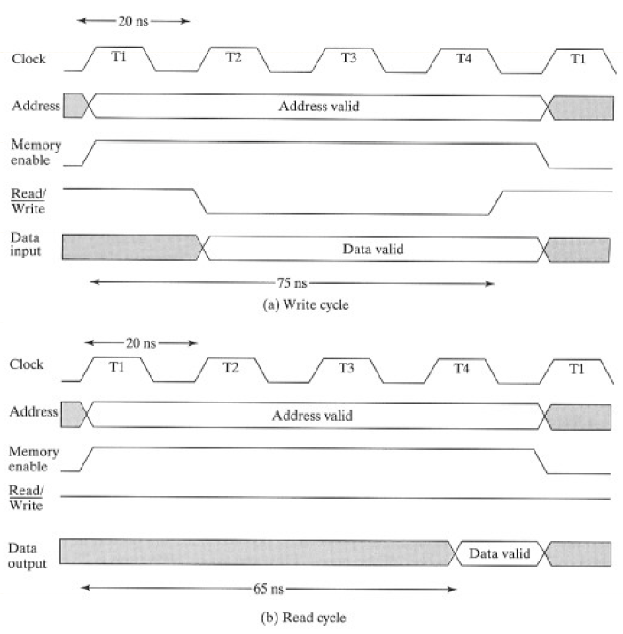
\includegraphics[scale=0.40]{../images/read-write-timing.png}
\label{read-write}
\end{center}
\end{figure}

\newline\newline
When the CPU is executing a read or write cycle, especially in this configuration, it will be busy waiting around for the slower memory to complete it's operation. At this point the CPU cannot conduct any transformations. For this reason, computer systems will often contain levels of much faster memory of differing sizes. We will discuss later is this chapter some techniques that assist us in minimizing this overhead. 
\newline\newline
At the circuit level, RAM can be \textbf{static} or \textbf{dynamic}. Static RAM uses an array of SR Latches \cite{SRLATCH} coupled with selection logic. Dynamic RAM actually use capacitor arrays which require periodic refresh. Static RAM typically has shorter read/write cycles but consumes more power than DRAM due to the requirement for constant charge. Economically, DRAM is cheaper to produce in larger quantities. SRAM my typically be found in on-chip cache, whereas DRAM is more commonly found in main system memory. 
\subsection{Memory Addressing}
As mentioned earlier, the physical address space of a computer is defined by the width of it's address bus. Components of the system will each have their own physical address space, which will be a sub-set of the entire address space. It is the responsibility of the \textbf{memory management unit} or MMU, to manage the mapping of \textbf{virtual} to physical addresses. In effect, the MMU provides a means for a program executing on the CPU to not have to worry about exactly where in the address space a particular piece of memory is mapped. This is a very important concept that you will see repeated in various flavours when we look at how operating systems work. 
\newline\newline
An MMU will divide the physical address space into \textbf{pages} of typically 4Kb in size. When a program references a particular location in its \textit{virtual address space} the MMU will use some translation mechanism to map to a physical address location. The size of the page allows the MMU to map virtual to physical address spaces, while keeping it's internal map relatively small and helping to keep the address translation fast. We will talk about these in more detail in later articles. 
\section{Execution of Instructions}
An \textit{instruction} is a sequence of bits that tells the CPU to perform a particular operation. The core instruction contains bit configurations that manipulate the control and data-paths of the CPU. Instructions may also have \textbf{operands} which define meta-data related to the instruction. Such meta-data includes location of data to be operated on in memory, or the actual data itself. In essence, programs are sequences of these instructions executed in some order by the CPU.
\subsection{Instruction Sets}
The instruction set is the set of machine-language primitives that can be directly executed on a processor. Historically, programmers would write programs directly using this set. However, in recent times, almost all except very specialist programming is done in much higher level languages. These languages are translated into the machine language that more directly encodes these instructions. This will typically happen at several layers of indirection before actual machine code is produced. Therefore, modern processors provide instruction sets that are designed to be translated to by compilers, and often contain specialist instructions that assist compilers in writing efficient programs. Nevertheless, these instructions can typically be categorized as follows. 
\begin{itemize}
\item ALU Instructions - Add, Subtract, Multiply
\item Memory Instructions - Load and Storing of data
\item Control Instructions - Conditional Branch, Call, Return, Interrupt 
\item Specialized Instructions - FPU Extensions, MMX Instructions
\end{itemize}
The transition to less human readable instruction sets occurred in parallel with the rise in popularity of RISC CPUs. A \textbf{reduced instruction set} CPU, as the name suggests, contains a smaller set of instructions. Program optimization, therefore, at the compiler level. In contrast, a \textbf{complex instruction set} CPU contains more complex operations that will be optimized at the hardware level. There is on-going debate as to which approach is the most desirable approach. Processors of the x86 range take the CISC approach, while PowerPC and some ARM processors will take the RISC approach. See \cite{RISC-CISC} for a comprehensive discussion.
\section{Fetch, Decode and Execute Cycle}
A \textbf{register} is a temporary storage location inside the CPU. The \textbf{register file} of the CPU will contain several general purpose registers of varying classes. Data registers are designed to contain data that is being operated on. Address registers are designed to contain locations in memory. Special purpose registers compliment the above file. The \textbf{program counter} points to the location in memory of the instruction which is to be next executed. A \textbf{memory data register} is often used as a buffer to memory data as it moves between the CPU and memory. Lastly, the \textbf{instruction register} contains the instruction that has just been fetched from memory.   






\bibliography{../biblio/techfundamentals.bib}{}
\bibliographystyle{plain}
\begin{center}
{\small \copyright  David Lynch 2012. Do not reproduce with written permission.}
\end{center}
\end{document}